\documentclass[hidelinks]{book}
\usepackage{Resources/UoBLab}
\usepackage[utf8]{inputenc}
\usepackage{amsmath}
\usepackage{subcaption}
\usepackage{hyperref}
\usepackage{graphicx}
\usepackage[textwidth=7in]{geometry}
\usepackage{algorithm}
\usepackage[
  backend=biber, maxparens=1002
]{biblatex}
\usepackage{fancyhdr}

\addbibresource{ref.bib}

\numberwithin{equation}{section}
\pubyear{2023}
\title{Optofluidic Bead Detection}
\author{Manav Seksaria}
\school{Centre for Quantum Information, Communication \& Computing, IIT Madras}
\date{\today}

\newcommand{\ts}{\textsuperscript}

\begin{document}

\maketitle

\pagestyle{fancy}
\fancyhead{}
\fancyfoot{}
\fancyhead[L]{Optofluidic Bead Detection}
\fancyhead[R]{CQuICC, IIT Madras}
\fancyfoot[L]{\it \small{Manav Seksaria}}
\fancyfoot[R]{\it \small{Nov'24}}

\section{Introduction}\label{sec:intro}
The problem at hand is given a video with frames such as below,

\begin{figure}[H]\label{fig:intro_beads}
  \centering
  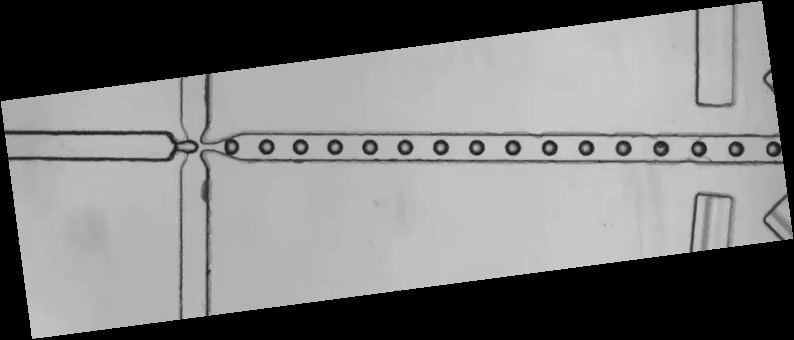
\includegraphics[width=\textwidth]{images_ppt/001.png}
  \caption{Array of circles}
\end{figure}

\noindent we need to find the mean radius and mean distance between the circles. Additionally, some circles may contian beads, which we need to detect and find, inside the bead, $r, \theta$ for each bead. We will follow the following general process.

\begin{itemize}
  \item \textbf{Step 1:} Getting basic properties of the circles
  \begin{itemize}
    \item Sobel Filter
    \item Coarse Hough Circle Transform (HCT)
    \item Find most likely radius $\pm \epsilon$
    \item Fine HCT with tuned params
    \item Find desired stats from obtained circles
  \end{itemize}
  \item \textbf{Step 2:} Detecting beads
  \begin{itemize}
    \item Find the luminance of each droplet by laser
    \item Find droplet with max luminance
    \item Image diff droplet with and without bead
    \item Find bead's parameters
  \end{itemize}
\end{itemize}

The main tool we'll use to do this is the Hough Circle Transform (HCT). We will first discuss the Hough Line Transform (HLT) to understand the basics of Hough Transforms. Skip this section to skip the mechanism of HCT, and take it as a given that it can detect circles.

\section{Preliminaries}\label{sec:prelim}
\subsection{Hough Line Transform}\label{ssec:hlt}
Consider a problem of detecting 'lines' in an image i.e given a set of points, we want to find the equation of the line that passes through the most number of points. For each point we create a parametrised family of lines in the Hesse normal form $r=x\cos \theta +y\sin \theta$.

\begin{figure}[H]
  \centering
  \includegraphics[width=\textwidth]{images_ppt/hough_line.png}
  \caption{Parametrised drawn through two points}
\end{figure}

For each point we then tabulate the data obtained by the lines that pass through it in the $r, \theta$ space.

\begin{table}[!ht]
    \centering
    \begin{tabular}{|l|l|l|l|l|l|}
    \hline
        $\theta$ & 15 & 30 & 45 & 60 & 75 \\ \hline
        $r_1$ (1\ts{st} Point) & 189 & 282 & 356 & 407 & 429 \\ \hline
        $r_2$ (2\ts{nd} Point) & 319 & 376 & 406 & 410 & 385 \\ \hline
    \end{tabular}
\end{table}

\noindent We can see from the data above that at $\theta=69^\circ$ and $r\approx 408.5$, we have two points that lie on the same line. This procedure can be run multiple times for each point and for varying levels of precision to give us all lines in the image. Similarly for circles, we take each point and a parametrised family of circles in the form $(x-a)^2 + (y-b)^2 = r^2$ and tabulate the data in the $a, b, r$ space.

\section{Step 1: Initial Parameters}\label{sec:step1}
\subsection{Course Scan Stage}\label{ssec:coarse}
Before running a course scan on the image we always find it convenient to convert it to grayscale and then run an edge filter on it.

\begin{figure}[H]
  \centering
  \includegraphics[width=\textwidth]{images_ppt/img.png}
  \caption{Original Image before Sobel Filter}
\end{figure}
%%
\begin{align*}
\mathbf{G}_x =\begin{bmatrix}
+1&0&-1\\+2&0&-2\\+1&0&-1
\end{bmatrix}*\mathbf {A} ,\,
\mathbf{G}_y =\begin{bmatrix}
+1&+2&+1\\0&0&0\\-1&-2&-1
\end{bmatrix}*\mathbf {A}
\end{align*}
%
\begin{figure}[H]
  \centering
  \includegraphics[width=\textwidth]{images_ppt/sobel.png}
  \caption{After Sobel Filter}
\end{figure}

We now set radius range $r\in [1, 20]$ and run a full sweep for all detected circles in order to determine how big the circles are.

\begin{figure}[H]
  \centering
  \includegraphics[width=\textwidth]{images_ppt/chct.png}
  \caption{Circles and some false positives}
\end{figure}

Considering that we know in our dataset, the desired droplets are all of similar size, we can run a modal filter to extract out mode radius $R$ (in this case 7px). Inital parameters for both the course and fine HCT are in Appendix \ref{appen:param}.

\subsection{Fine Scan Stage}\label{ssec:fine}
With the new guess radius we run HCT again with more tuned parameters and a 10\% error margin to find the desired circles i.e. $R\in [R-\epsilon, R+\epsilon]$.

\begin{figure}[H]
  \centering
  \includegraphics[width=\textwidth]{images_ppt/fhct.png}
  \caption{Circles and some false negatives}
\end{figure}

With a more accurate guess we're ensured to pick out most of the desired circles with few misses. Since now we expect all beads to be in a straight line, any deviation in the '$y$' values of is useless information, (146, 147, 148) to us mean the same thing. Therefore we normalise the $y$ values as $y \rightarrow \text{round}(y/R) \cdot R$.

Then once again we pick out all the modal radius and modal $y$ values to pick out all our circles. Giving us a list of circles with some $x$ values and fixed $y, r$ values (in our case $y=147, r=7$px).
%
\begin{align*}
  X_i \in [266, 301, 336, 371, 406, 441, 476, 511, 546, 623, 665, 700, 735, 770]
\end{align*}

We can then find $\frac{X_{i+1} - X_i}R - 2\, \forall\, X_i$ to find the mean distance between the circles, textit{from edge to edge} and not from center to center, giving us a list of intra-droplet distances.
%
\begin{align*}
\frac{X_{i+1} - X_i}R - 2 \in [3, 3, 3, 3, 3, 3, 3, 3, 9, 4, 3, 3, 3]
\end{align*}

Finally we can see that the expected mean distance between the circles is $3R$ with the $R=7$px.

\subsection{Post Processing}\label{ssec:post}
So far we have generated all the information we have from just the first frame. We can now split the video into multiple frames and run the following process:

\begin{itemize}
  \item Select a small $12\times12$ window in the center of the image
  \item From the first image matrix $M_1$, find image distances for next 50 frames
  \item $||M_1 - M_i||_F$ then indicates images distance
  \item Looping over first 50 frames find the minimal distance
\end{itemize}

This procedure will give us the 'droplet' frequency of the video i.e. for a given area, how long does it take (in frames) for the next bead to exactly replace the previous one.

\section{Step 2: Bead Detection}\label{sec:step2}
\subsection{Luminance Detection}\label{ssec:lum}
We pick another square where the laser and measure the luminance of each frame. Sample images as shown

\begin{figure}[H]
  \centering
  \begin{subfigure}{.5\textwidth}
    \centering
    \includegraphics[width=.9\linewidth]{images_ppt/laser_hit.png}
    \caption{Laser hits Droplet}
  \end{subfigure}%
  \begin{subfigure}{.5\textwidth}
    \centering
    \includegraphics[width=.9\linewidth]{images_ppt/laser_null.png}
    \caption{Laser misses Droplet}
  \end{subfigure}
\end{figure}

We can then find the droplet with the maximum luminance and then find the difference between the two images to find the bead. Luminance hear is defined as sum of brightness of all pixels brighter than a threshold. With this we will receive list each frame with its associated luminance. We can then pick out all frames with luminance higher than one standard deviation. We now have a new list that looks like
%
\begin{align*}
  \text{Luminance}_i \in [99, 125, 127, 90, 96, 154, 224, 249, 216, 171, 107] \\
  \text{Frames}_i \in [23, 24, 25, 26, 74, 75, 76, 77, 78, 79, 80]
\end{align*}

We can clearly see these are ranges of frames from where the droplet enters to when the droplet exits the line of the laser. For each of these ranges we can then pick out the frame with the maximum luminance giving us
%
\begin{align*}
  \text{Frames}_i \in [25, 77] \\
  \text{Luminance}_i \in [127, 249]
\end{align*}

This list will now give us the frames where the droplet is in the laser line. The largest of these values will contain the bead, as shown in the image below.

\begin{figure}[H]
  \centering
  \begin{subfigure}{.5\textwidth}
    \centering
    \includegraphics[width=.9\linewidth]{images_ppt/laser_hit.png}
    \caption{Bead not in Laser Line}
  \end{subfigure}%
  \begin{subfigure}{.5\textwidth}
    \centering
    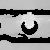
\includegraphics[width=.9\linewidth]{images_ppt/laser_bead.png}
    \caption{Bead in Laser Line}
  \end{subfigure}
\end{figure}

\subsection{Walking back on $y$-axis}\label{ssec:bead}
We now have a frame with a bead in it, a frame without a bead in it, the intra-bead distance and the bead frequency. In the original image now, we can walk back on the $y$-axis by 1 bead distance to go exactly out of the laser line, and then also go back 1 time period of the bead to encounter our detected bead. We can then take two images one with bead and one without bead as shown below.

\begin{figure}[H]
  \centering
  \includegraphics[width=\textwidth]{images_ppt/woutw.png}
  \caption{Without and with bead}
\end{figure}

We now run a small gaussian filter on the two images to avoid image artefacts (see Appendix \ref{appen:gaussian}) and then take image difference $M_{\text{bead}} - M_{\text{no bead}}$ to get the bead only. We can then find the brightest 3x3 patch in the image and mark the brightest pixel as the center of the bead

\begin{figure}[H]
  \centering
  \includegraphics[width=\textwidth]{images_ppt/diff.png}
  \caption{Bead Detected as a bright spot. Line from center (red) to bead (blue)}
\end{figure}

We can use center of droplet as origin and find the $(r, \theta)$ for the bead. This process can be repeated for all beads in the video to get the desired results.


\section{Appendix}\label{sec:app}
\subsection{HCT Parameters}\label{appen:param}
\textbf{Course HCT Parameters:}
\begin{itemize}
  \item Min Center Distance = $\text{Image Height} / 8$
  \item HCT Tuning params = $100, 15$
  \item Radius Range = $[1, 20]$
\end{itemize}

\textbf{Fine HCT Parameters:}
\begin{itemize}
  \item Min Center Distance = $\text{Image Height} / 2 * (R + E)$
  \item HCT Tuning params = $100, 10$
  \item Radius Range = $[R - E, R + E]$
\end{itemize}

\subsection{Gaussian Filter}\label{appen:gaussian}
It is standard practice in image processing to use a gaussian filter to smooth out the image before running filters to

\begin{itemize}
  \item Remove dead pixels
  \item Avoid Mura effect
  \item Avoid compression artefacts
\end{itemize}

\begin{figure}[H]
  \centering
  \includegraphics[width=\textwidth]{images_ppt/mura.webp}
  \caption{Mura Effect where all the pixels are not uniform. \textit{source: roadtovr.com}}
\end{figure}

\begin{figure}[H]
  \centering
  \includegraphics[width=\textwidth]{images_ppt/banding.webp}
  \caption{Compression artefacts in an image. \textit{source: Netflix Tech Blog}}
\end{figure}

\nocite{*}
\printbibliography

\end{document}
